\documentclass[12pt,a4paper]{article}
\usepackage{pgfplots}
\usepackage{tikz}

\usepackage[font=small,labelfont=bf]{caption}

\begin{document}


\begin{figure}
\caption*{Sequences 59, 10 CPUS}
\begin{minipage}{0.49\textwidth}
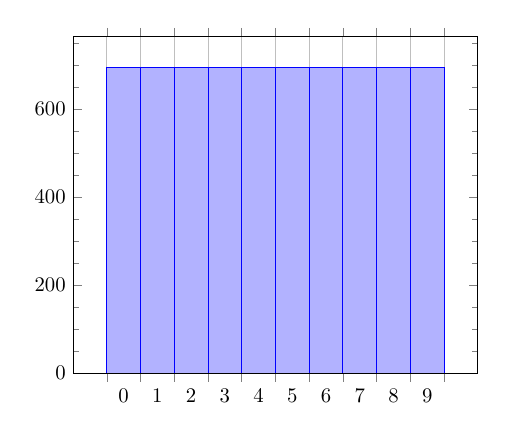
\begin{tikzpicture}[scale=0.75]
  \begin{axis}[ybar interval, ymax=765,ymin=0, minor y tick num = 3]
    \addplot coordinates { (0,695) (1,695) (2,695) (3,696) (4,695) (5,695) (6,695) (7,695) (8,695) (9,695) (10, 348) };
  \end{axis}
\end{tikzpicture}
\caption*{Sites repartition with Kassian}
\end{minipage}
\begin{minipage}{0.49\textwidth}
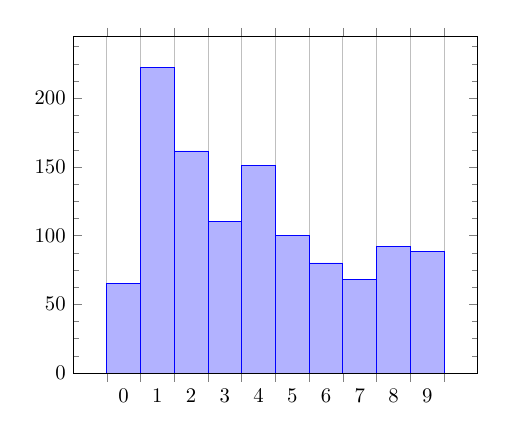
\begin{tikzpicture}[scale=0.75]
  \begin{axis}[ybar interval, ymax=244.731,ymin=0, minor y tick num = 3]
    \addplot coordinates { (0,64.9655) (1,222.483) (2,161.586) (3,110.172) (4,150.759) (5,100.052) (6,80.069) (7,68.2414) (8,91.8793) (9,88.569) (10, 111.241) };
  \end{axis}
\end{tikzpicture}
\caption*{PLF-cost repartition with Kassian}
\end{minipage}
\begin{minipage}{0.49\textwidth}
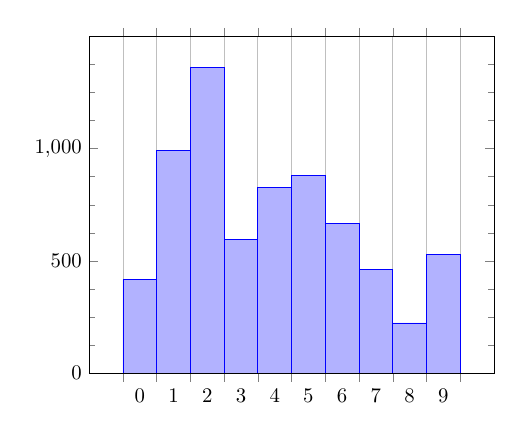
\begin{tikzpicture}[scale=0.75]
  \begin{axis}[ybar interval, ymax=1499,ymin=0, minor y tick num = 3]
    \addplot coordinates { (0,417) (1,991) (2,1363) (3,595) (4,826) (5,879) (6,666) (7,461) (8,223) (9,530) (10, 681) };
  \end{axis}
\end{tikzpicture}
\caption*{Sites repartition with Weighted}
\end{minipage}
\begin{minipage}{0.49\textwidth}
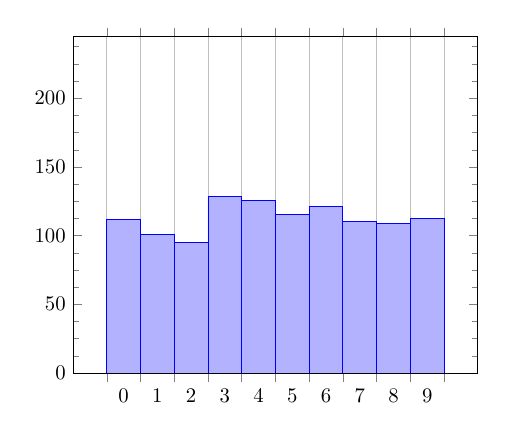
\begin{tikzpicture}[scale=0.75]
  \begin{axis}[ybar interval, ymax=244.731,ymin=0, minor y tick num = 3]
    \addplot coordinates { (0,111.586) (1,100.655) (2,94.7759) (3,128.793) (4,125.259) (5,115.569) (6,121.5) (7,110.379) (8,109.017) (9,112.345) (10, 111.241) };
  \end{axis}
\end{tikzpicture}
\caption*{PLM-cost repartition with Weighted}
\end{minipage}
\end{figure}




\begin{figure}
\caption*{Sequences 128, 10 CPUS}
\begin{minipage}{0.49\textwidth}
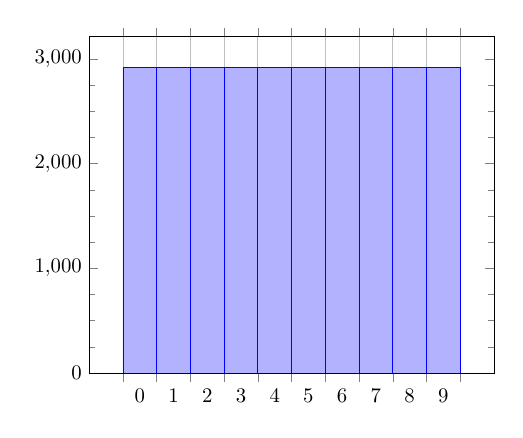
\begin{tikzpicture}[scale=0.75]
  \begin{axis}[ybar interval, ymax=3212,ymin=0, minor y tick num = 3]
    \addplot coordinates { (0,2919) (1,2919) (2,2920) (3,2920) (4,2920) (5,2920) (6,2920) (7,2920) (8,2920) (9,2920) (10, 1460) };
  \end{axis}
\end{tikzpicture}
\caption*{Sites repartition with Kassian}
\end{minipage}
\begin{minipage}{0.49\textwidth}
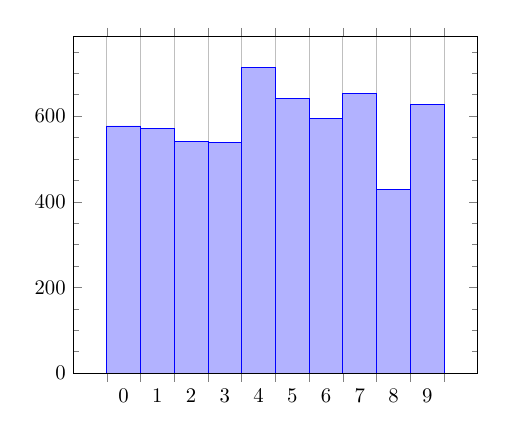
\begin{tikzpicture}[scale=0.75]
  \begin{axis}[ybar interval, ymax=785.365,ymin=0, minor y tick num = 3]
    \addplot coordinates { (0,576.961) (1,571.921) (2,540.811) (3,537.354) (4,713.969) (5,640.764) (6,593.866) (7,652.701) (8,428.433) (9,627.551) (10, 356.984) };
  \end{axis}
\end{tikzpicture}
\caption*{PLF-cost repartition with Kassian}
\end{minipage}
\begin{minipage}{0.49\textwidth}
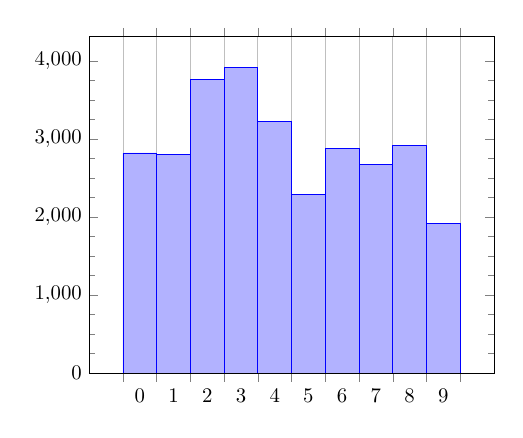
\begin{tikzpicture}[scale=0.75]
  \begin{axis}[ybar interval, ymax=4309,ymin=0, minor y tick num = 3]
    \addplot coordinates { (0,2820) (1,2801) (2,3757) (3,3918) (4,3229) (5,2289) (6,2880) (7,2668) (8,2918) (9,1918) (10, 1959) };
  \end{axis}
\end{tikzpicture}
\caption*{Sites repartition with Weighted}
\end{minipage}
\begin{minipage}{0.49\textwidth}
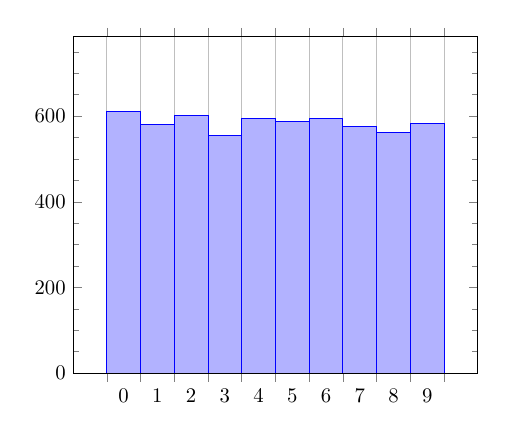
\begin{tikzpicture}[scale=0.75]
  \begin{axis}[ybar interval, ymax=785.365,ymin=0, minor y tick num = 3]
    \addplot coordinates { (0,610.937) (1,579.89) (2,601.165) (3,554.661) (4,594.291) (5,588.417) (6,594.472) (7,576.843) (8,562.283) (9,582.874) (10, 356.984) };
  \end{axis}
\end{tikzpicture}
\caption*{PLM-cost repartition with Weighted}
\end{minipage}
\end{figure}


\begin{figure}
\caption*{Sequences 404, 10 CPUS}
\begin{minipage}{0.49\textwidth}
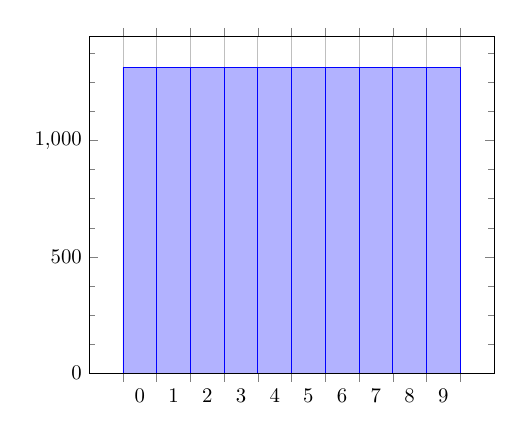
\begin{tikzpicture}[scale=0.75]
  \begin{axis}[ybar interval, ymax=1447,ymin=0, minor y tick num = 3]
    \addplot coordinates { (0,1315) (1,1315) (2,1316) (3,1316) (4,1316) (5,1316) (6,1316) (7,1316) (8,1316) (9,1316) (10, 658) };
  \end{axis}
\end{tikzpicture}
\caption*{Sites repartition with Kassian}
\end{minipage}
\begin{minipage}{0.49\textwidth}
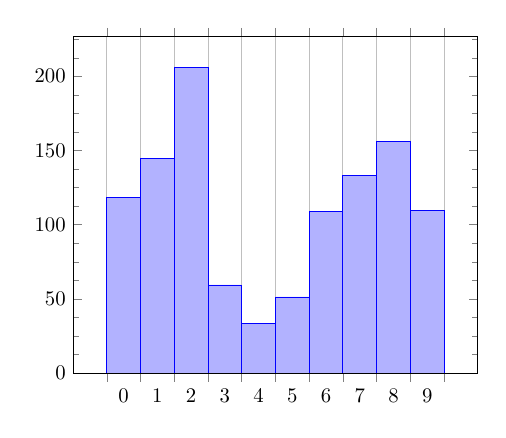
\begin{tikzpicture}[scale=0.75]
  \begin{axis}[ybar interval, ymax=226.641,ymin=0, minor y tick num = 3]
    \addplot coordinates { (0,118.342) (1,144.489) (2,206.037) (3,59.3226) (4,33.3896) (5,51.2308) (6,108.935) (7,133.412) (8,155.759) (9,109.797) (10, 103.019) };
  \end{axis}
\end{tikzpicture}
\caption*{PLF-cost repartition with Kassian}
\end{minipage}
\begin{minipage}{0.49\textwidth}
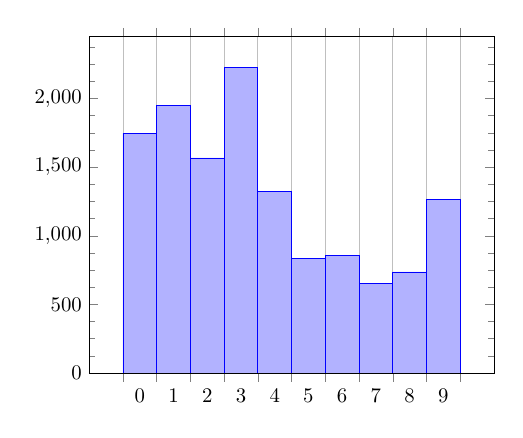
\begin{tikzpicture}[scale=0.75]
  \begin{axis}[ybar interval, ymax=2450,ymin=0, minor y tick num = 3]
    \addplot coordinates { (0,1747) (1,1952) (2,1567) (3,2228) (4,1323) (5,833) (6,856) (7,652) (8,736) (9,1264) (10, 1114) };
  \end{axis}
\end{tikzpicture}
\caption*{Sites repartition with Weighted}
\end{minipage}
\begin{minipage}{0.49\textwidth}
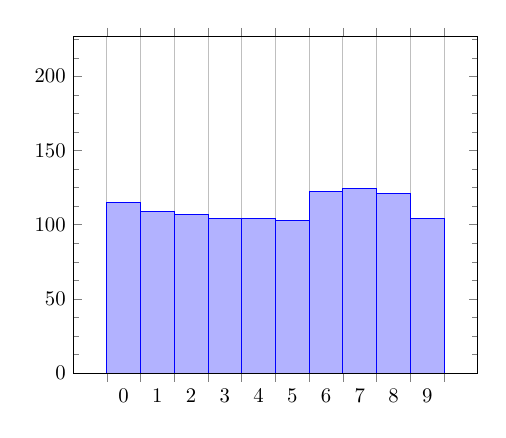
\begin{tikzpicture}[scale=0.75]
  \begin{axis}[ybar interval, ymax=226.641,ymin=0, minor y tick num = 3]
    \addplot coordinates { (0,115.03) (1,108.95) (2,106.943) (3,104.211) (4,104.457) (5,103.01) (6,122.099) (7,124.233) (8,120.794) (9,104.146) (10, 103.019) };
  \end{axis}
\end{tikzpicture}
\caption*{PLM-cost repartition with Weighted}
\end{minipage}
\end{figure}


\begin{figure}
\caption*{Sequences proteins 94, 200 CPUS}
\begin{minipage}{0.49\textwidth}
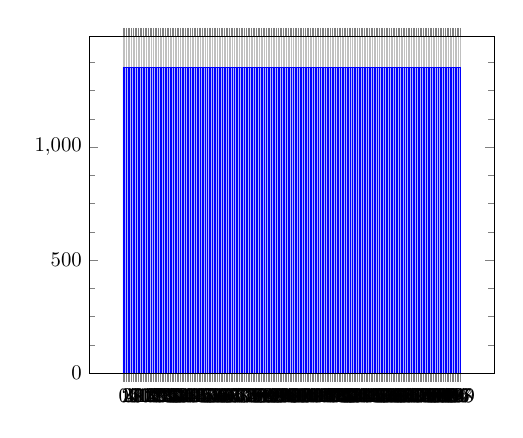
\begin{tikzpicture}[scale=0.75]
  \begin{axis}[ybar interval, ymax=1488,ymin=0, minor y tick num = 3]
    \addplot coordinates { (0,1353) (1,1353) (2,1353) (3,1352) (4,1352) (5,1352) (6,1352) (7,1352) (8,1352) (9,1352) (10,1352) (11,1352) (12,1352) (13,1352) (14,1352) (15,1352) (16,1352) (17,1352) (18,1352) (19,1352) (20,1352) (21,1352) (22,1352) (23,1353) (24,1353) (25,1353) (26,1353) (27,1353) (28,1353) (29,1353) (30,1353) (31,1353) (32,1353) (33,1353) (34,1353) (35,1353) (36,1353) (37,1353) (38,1353) (39,1353) (40,1353) (41,1353) (42,1353) (43,1353) (44,1353) (45,1353) (46,1353) (47,1353) (48,1353) (49,1353) (50,1353) (51,1353) (52,1353) (53,1353) (54,1353) (55,1353) (56,1353) (57,1353) (58,1353) (59,1353) (60,1353) (61,1353) (62,1353) (63,1353) (64,1353) (65,1353) (66,1353) (67,1353) (68,1353) (69,1353) (70,1353) (71,1353) (72,1353) (73,1353) (74,1353) (75,1353) (76,1353) (77,1353) (78,1353) (79,1353) (80,1353) (81,1353) (82,1353) (83,1353) (84,1353) (85,1353) (86,1353) (87,1353) (88,1353) (89,1353) (90,1353) (91,1353) (92,1353) (93,1353) (94,1353) (95,1353) (96,1353) (97,1353) (98,1353) (99,1353) (100,1353) (101,1353) (102,1353) (103,1353) (104,1353) (105,1353) (106,1353) (107,1353) (108,1353) (109,1353) (110,1353) (111,1353) (112,1353) (113,1353) (114,1353) (115,1353) (116,1353) (117,1353) (118,1353) (119,1353) (120,1353) (121,1353) (122,1353) (123,1353) (124,1353) (125,1353) (126,1353) (127,1353) (128,1353) (129,1353) (130,1353) (131,1353) (132,1353) (133,1353) (134,1353) (135,1353) (136,1353) (137,1353) (138,1353) (139,1353) (140,1353) (141,1353) (142,1353) (143,1353) (144,1353) (145,1353) (146,1353) (147,1353) (148,1353) (149,1353) (150,1353) (151,1353) (152,1353) (153,1353) (154,1353) (155,1353) (156,1353) (157,1353) (158,1353) (159,1353) (160,1353) (161,1353) (162,1353) (163,1353) (164,1353) (165,1353) (166,1353) (167,1353) (168,1353) (169,1353) (170,1353) (171,1353) (172,1353) (173,1353) (174,1353) (175,1353) (176,1353) (177,1353) (178,1353) (179,1353) (180,1353) (181,1353) (182,1353) (183,1353) (184,1353) (185,1353) (186,1353) (187,1353) (188,1353) (189,1353) (190,1353) (191,1353) (192,1353) (193,1353) (194,1353) (195,1353) (196,1353) (197,1353) (198,1353) (199,1353) (200, 676) };
  \end{axis}
\end{tikzpicture}
\caption*{Sites repartition with Kassian}
\end{minipage}
\begin{minipage}{0.49\textwidth}
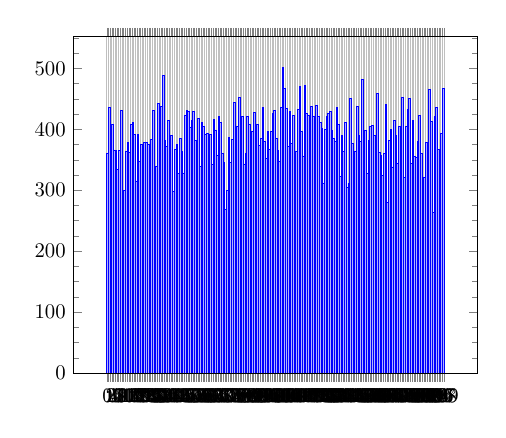
\begin{tikzpicture}[scale=0.75]
  \begin{axis}[ybar interval, ymax=551.999,ymin=0, minor y tick num = 3]
    \addplot coordinates { (0,361.215) (1,436.409) (2,370.505) (3,407.86) (4,366.161) (5,364.57) (6,334.215) (7,365.72) (8,431.032) (9,283.441) (10,299.559) (11,363.892) (12,378.817) (13,362.43) (14,408.28) (15,411.57) (16,392.108) (17,315.247) (18,392.29) (19,346.828) (20,375.355) (21,344.258) (22,378.548) (23,377.946) (24,375.527) (25,361.376) (26,383.237) (27,430.226) (28,323.688) (29,338.796) (30,442) (31,387) (32,437.774) (33,487.957) (34,381.323) (35,372.376) (36,414.129) (37,369.656) (38,390.645) (39,298.022) (40,367.312) (41,374.43) (42,327.462) (43,384.495) (44,363.452) (45,328.161) (46,422.527) (47,430.817) (48,429.495) (49,403.914) (50,413.86) (51,428.849) (52,381) (53,365.097) (54,417.108) (55,338.903) (56,411.935) (57,405.086) (58,391.172) (59,393.968) (60,356.656) (61,392.151) (62,342.882) (63,415.72) (64,398.989) (65,357.462) (66,421.28) (67,411.387) (68,360.914) (69,345.645) (70,269.086) (71,300.237) (72,386.742) (73,345.258) (74,383.505) (75,443.871) (76,382.032) (77,404.677) (78,452.409) (79,345.86) (80,421.785) (81,343.086) (82,360.656) (83,420.462) (84,407.978) (85,387.495) (86,397.065) (87,428.258) (88,352.161) (89,407.86) (90,373.387) (91,384.516) (92,436.312) (93,379.753) (94,352.344) (95,396.817) (96,366.656) (97,395.978) (98,426.796) (99,431.043) (100,385.634) (101,365.065) (102,346.527) (103,436.462) (104,501.817) (105,466.548) (106,434.796) (107,372) (108,428.602) (109,377.054) (110,422.989) (111,360.29) (112,363.398) (113,432.613) (114,470.086) (115,397.194) (116,356.204) (117,472.796) (118,426.312) (119,423.29) (120,328.731) (121,437.57) (122,421.914) (123,403.774) (124,439.57) (125,420.548) (126,411.505) (127,401.398) (128,311.097) (129,399.054) (130,421.591) (131,426.258) (132,429.688) (133,398.032) (134,385.527) (135,379.559) (136,436.172) (137,407.892) (138,321.935) (139,390.075) (140,363.441) (141,410.978) (142,303.914) (143,311.978) (144,450.151) (145,377.495) (146,363.011) (147,364.548) (148,437.925) (149,390.699) (150,379.452) (151,482.505) (152,363.065) (153,397.462) (154,327.968) (155,382.548) (156,405.215) (157,407.054) (158,390.075) (159,368.591) (160,458.398) (161,362.505) (162,356.613) (163,324.032) (164,359.699) (165,440.796) (166,279.785) (167,381.247) (168,399.71) (169,338.226) (170,415.14) (171,389.613) (172,343.312) (173,404.387) (174,369.43) (175,452.613) (176,321.656) (177,404.677) (178,432.591) (179,451.194) (180,344.194) (181,414.688) (182,355.258) (183,354.151) (184,380.72) (185,423.172) (186,360.785) (187,305.785) (188,320.624) (189,378.161) (190,343.72) (191,465.806) (192,412.742) (193,263.29) (194,420.925) (195,436.075) (196,367.398) (197,305.032) (198,392.505) (199,466.634) (200, 250.909) };
  \end{axis}
\end{tikzpicture}
\caption*{PLF-cost repartition with Kassian}
\end{minipage}
\begin{minipage}{0.49\textwidth}
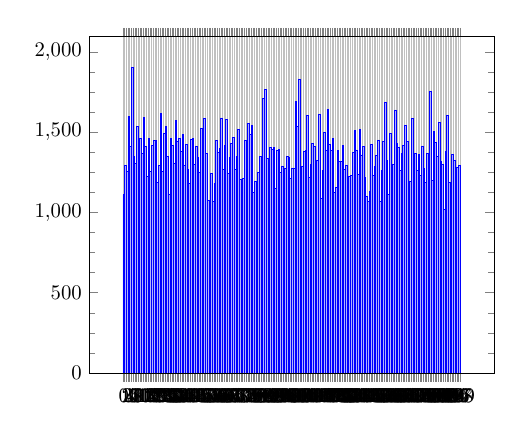
\begin{tikzpicture}[scale=0.75]
  \begin{axis}[ybar interval, ymax=2094,ymin=0, minor y tick num = 3]
    \addplot coordinates { (0,1110) (1,1291) (2,1253) (3,1598) (4,1412) (5,1904) (6,1346) (7,1304) (8,1534) (9,1212) (10,1460) (11,1369) (12,1591) (13,1411) (14,1225) (15,1460) (16,1257) (17,1418) (18,1448) (19,1446) (20,1184) (21,1291) (22,1616) (23,1255) (24,1492) (25,1537) (26,1348) (27,1110) (28,1460) (29,1415) (30,1305) (31,1572) (32,1439) (33,1463) (34,1377) (35,1483) (36,1293) (37,1424) (38,1266) (39,1181) (40,1456) (41,1458) (42,1297) (43,1412) (44,1344) (45,1251) (46,1520) (47,1256) (48,1586) (49,1366) (50,1077) (51,995) (52,1240) (53,1067) (54,1183) (55,1446) (56,1374) (57,1397) (58,1588) (59,1268) (60,1419) (61,1581) (62,1242) (63,1342) (64,1427) (65,1465) (66,1265) (67,1351) (68,1517) (69,1203) (70,1187) (71,1211) (72,1447) (73,1385) (74,1554) (75,1483) (76,1539) (77,1122) (78,1195) (79,1098) (80,1250) (81,1347) (82,1228) (83,1708) (84,1766) (85,1338) (86,1328) (87,1403) (88,1393) (89,1405) (90,1147) (91,1383) (92,1391) (93,1250) (94,1289) (95,1142) (96,1273) (97,1347) (98,1342) (99,1209) (100,1277) (101,1272) (102,1691) (103,1538) (104,1831) (105,1261) (106,1287) (107,1378) (108,1389) (109,1601) (110,1216) (111,1299) (112,1430) (113,1413) (114,1312) (115,1325) (116,1613) (117,1085) (118,1263) (119,1501) (120,1387) (121,1643) (122,1425) (123,1386) (124,1461) (125,1122) (126,1155) (127,1384) (128,1315) (129,1318) (130,1419) (131,1270) (132,1295) (133,1098) (134,1222) (135,1228) (136,1376) (137,1508) (138,1389) (139,1237) (140,1516) (141,1358) (142,1408) (143,1216) (144,1102) (145,1070) (146,1133) (147,1423) (148,1228) (149,1289) (150,1355) (151,1451) (152,1068) (153,1264) (154,1439) (155,1688) (156,1326) (157,1110) (158,1491) (159,1153) (160,1300) (161,1638) (162,1428) (163,1404) (164,1263) (165,1369) (166,1417) (167,1541) (168,1439) (169,1114) (170,1193) (171,1587) (172,1210) (173,1369) (174,1263) (175,1360) (176,1232) (177,1414) (178,1273) (179,1187) (180,1369) (181,1249) (182,1751) (183,1201) (184,1502) (185,1438) (186,1347) (187,1560) (188,1316) (189,1300) (190,1016) (191,1381) (192,1605) (193,1184) (194,1111) (195,1361) (196,1321) (197,1174) (198,1279) (199,1293) (200, 952) };
  \end{axis}
\end{tikzpicture}
\caption*{Sites repartition with Weighted}
\end{minipage}
\begin{minipage}{0.49\textwidth}
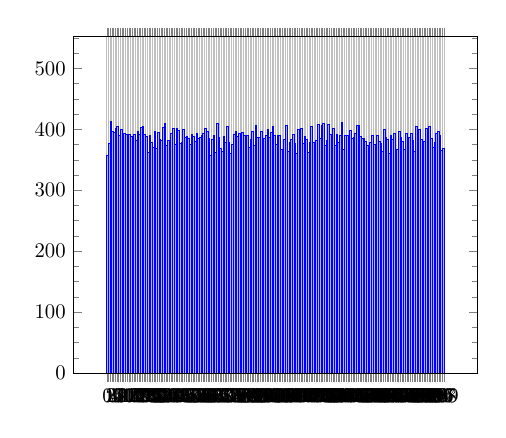
\begin{tikzpicture}[scale=0.75]
  \begin{axis}[ybar interval, ymax=551.999,ymin=0, minor y tick num = 3]
    \addplot coordinates { (0,357.505) (1,376.108) (2,413.688) (3,396.473) (4,395.484) (5,401.656) (6,405.172) (7,390.495) (8,399.151) (9,379.108) (10,392.86) (11,392.323) (12,377.591) (13,392.409) (14,388.753) (15,362.591) (16,392.086) (17,382.161) (18,397.312) (19,391.43) (20,403.753) (21,404.731) (22,391.108) (23,388.204) (24,362.118) (25,390.452) (26,378.452) (27,369.731) (28,396.677) (29,368.914) (30,395.215) (31,382.914) (32,381.957) (33,402.914) (34,409.097) (35,373.591) (36,381.849) (37,369.925) (38,392.892) (39,402.075) (40,375.108) (41,402.172) (42,398.323) (43,376.344) (44,378.634) (45,399.301) (46,386.355) (47,389.108) (48,385.882) (49,374.796) (50,391.57) (51,388.075) (52,380.957) (53,392.71) (54,385.72) (55,386.602) (56,390.28) (57,393.731) (58,401.355) (59,395.903) (60,384.473) (61,357.505) (62,383.796) (63,390.301) (64,361.527) (65,409.602) (66,386.011) (67,369.355) (68,364.054) (69,388.602) (70,378.376) (71,404.333) (72,378.71) (73,361.215) (74,375.151) (75,391.301) (76,395.946) (77,387.946) (78,393.344) (79,378.097) (80,394.581) (81,390.742) (82,389.054) (83,389.86) (84,370.946) (85,383.344) (86,396.849) (87,373.022) (88,407.215) (89,387.075) (90,386.118) (91,396.065) (92,383.495) (93,384.387) (94,389.301) (95,399.194) (96,386.194) (97,394.387) (98,405.226) (99,390.57) (100,375.731) (101,389.871) (102,389.538) (103,367.495) (104,366.968) (105,382.978) (106,406.806) (107,363.57) (108,378.505) (109,382.774) (110,391.194) (111,377.108) (112,360.344) (113,400.473) (114,383.527) (115,401.914) (116,376.968) (117,388.624) (118,383.366) (119,361.516) (120,377.86) (121,404.978) (122,378.28) (123,377.613) (124,381.581) (125,407.591) (126,385.258) (127,405.763) (128,409.774) (129,374.151) (130,381.828) (131,407.409) (132,390.914) (133,391.925) (134,400.957) (135,373.957) (136,392.344) (137,378.839) (138,389.989) (139,410.699) (140,367.806) (141,390.409) (142,390.097) (143,380.978) (144,398.473) (145,385.376) (146,387.129) (147,392.86) (148,406.634) (149,405.699) (150,388.011) (151,385.613) (152,384.753) (153,379.871) (154,373.753) (155,359.312) (156,378.215) (157,389.914) (158,375.43) (159,371.161) (160,390.688) (161,380.581) (162,377.602) (163,362.935) (164,400.032) (165,386.409) (166,382.774) (167,360.516) (168,389.548) (169,384.204) (170,392.839) (171,367.419) (172,366.806) (173,397.215) (174,386.581) (175,380.226) (176,367.774) (177,392.645) (178,383.871) (179,387.054) (180,392.957) (181,381.763) (182,364.333) (183,404.14) (184,375.935) (185,399.914) (186,383.849) (187,362.882) (188,380.075) (189,401.892) (190,394.376) (191,404.72) (192,384.882) (193,370.129) (194,378.011) (195,392.677) (196,396.71) (197,390.419) (198,365.882) (199,368.484) (200, 250.909) };
  \end{axis}
\end{tikzpicture}
\caption*{PLM-cost repartition with Weighted}
\end{minipage}


\end{figure}
                

\end{document}